% A document to start writing in.
%
% Everything below is here because you will want it within the first hour:
% maths, a figure, a table, a citation.  Delete what you do not need -- none
% of it is load-bearing.  When you settle on a journal or a handbook, give
% Claude that document and it will reshape this around the real rules.

\documentclass[11pt]{article}

\usepackage[T1]{fontenc}
\usepackage{lmodern}                      % a proper text font, not the 1980s default
\usepackage[margin=1in]{geometry}
\usepackage{parskip}                      % blank lines between paragraphs
\usepackage{microtype}                    % quietly better spacing

\usepackage{amsmath, amssymb}             % maths
\usepackage{graphicx}                     % figures
\usepackage{booktabs}                     % tables that look like a journal's
\usepackage{siunitx}                      % numbers and units, done properly
\usepackage{tikz}                         % drawings, used for the example figure

\usepackage[backend=biber, style=numeric, sorting=none]{biblatex}
\addbibresource{references.bib}

\usepackage{hyperref}                     % always last
\hypersetup{colorlinks, linkcolor=black, citecolor=black, urlcolor=blue}

\title{A Working Title}
\author{Your Name}
\date{\today}

\begin{document}
\maketitle

\begin{abstract}
  One paragraph saying what the work is, what you did, and what you found.
  Write it last.
\end{abstract}

\section{Introduction}
\label{sec:introduction}

Start here.  A sentence with a citation looks like this~\cite{knuth1984}, and
a reference to another part of the document looks like
Section~\ref{sec:results}.

Inline maths sits in dollars: the energy gap $\Delta E$ between two states.
Numbers with units go through \texttt{siunitx}, which handles the spacing and
the minus signs: \SI{2.7}{\electronvolt}, \SI{1.5e-12}{\second}.

\section{Results}
\label{sec:results}

A numbered equation, which you can refer back to as
Equation~\eqref{eq:example}:

\begin{equation}
  \label{eq:example}
  i\hbar \frac{\partial}{\partial t} \Psi(\mathbf{r}, t)
    = \hat{H}\, \Psi(\mathbf{r}, t).
\end{equation}

\begin{figure}[htbp]
  \centering
  % Drawn here so this document compiles before you have added any images.
  % To use a real figure instead: drag the file onto the figures folder in
  % the file list, then swap these three lines for the commented one below.
  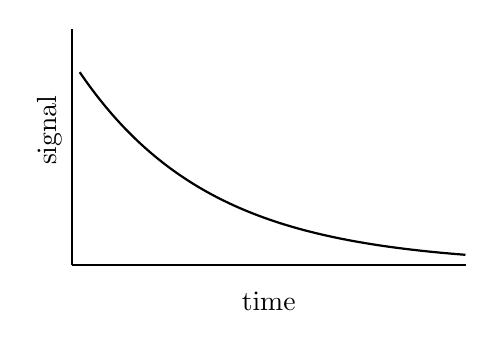
\begin{tikzpicture}
    \draw[thick] (0,0) -- (5,0) node[midway, below=6pt] {time};
    \draw[thick] (0,0) -- (0,3) node[midway, above=6pt, rotate=90] {signal};
    \draw[thick, smooth, domain=0.1:5, samples=60]
      plot (\x, {2.6 * exp(-0.6 * \x)});
  \end{tikzpicture}
  % \includegraphics[width=0.6\linewidth]{figures/your-image.png}
  \caption{What the reader should notice, in one sentence. A caption is read
    far more often than the paragraph that refers to it.}
  \label{fig:example}
\end{figure}

Figure~\ref{fig:example} shows the shape of the thing.  Table~\ref{tab:example}
gives the numbers behind it.

\begin{table}[htbp]
  \centering
  \caption{Rules for a readable table: no vertical lines, three horizontal
    ones, and numbers aligned on the decimal point.}
  \label{tab:example}
  \sisetup{table-format = 1.2}
  \begin{tabular}{l S S}
    \toprule
    State & {Energy (\si{\electronvolt})} & {Lifetime (\si{\pico\second})} \\
    \midrule
    First  & 3.41 & 1.20 \\
    Second & 4.07 & 0.35 \\
    \bottomrule
  \end{tabular}
\end{table}

\section{Discussion}

What the results mean, and what they do not.

\printbibliography

\end{document}
